\documentclass{article}

\usepackage{amsmath}
\usepackage{caption}
\usepackage[a4paper, margin=1in]{geometry}
\usepackage{graphicx}
\usepackage{parskip}
\usepackage{tabularx}

\setlength{\extrarowheight}{.5em}
\newcommand{\angstrom}{\mbox{\normalfont\AA}}

\title{Stellar Populations Coursework}
\author{Calvin Sykes}
\date{\today}

\begin{document}

\maketitle

\section*{Question 1}

Salpeter initial mass function is:
\begin{equation}
  N(M)\mathrm{d}M=M^{-\alpha}\mathrm{d}M\mbox{ with }\alpha=-2.35
\end{equation}

The mass-lifetime relations for main-sequence and red giant branch stars are assumed to be:
\begin{align}
  \tau_{\mathrm{MS}}(M)&=10^{10}\left(\frac{M}{M_\odot}\right)^{-2.5}\;\mathrm{yrs}\\
  \tau_{\mathrm{RGB}}(M)&=10^{9}\left(\frac{M}{M_\odot}\right)^{-4.0}\;\mathrm{yrs}
\end{align}

\underline{\bf{(a)} Number fractions of surviving stars}

The maximum surviving stellar mass at $T=10\;\mathrm{Gyr}$ $M_{\mathrm{max}}$ is defined by:
\begin{equation}
  \tau_{\mathrm{MS}}(M_{\mathrm{max}})+\tau_{\mathrm{RGB}}(M_{\mathrm{max}})=10\;\mathrm{Gyr}
\end{equation}

This identity can be solved numerically to yield $M_{\mathrm{max}}=1.037\,M_\odot$.

The total number of stars with mass $M$ such that $M_1<M<M_2$ is:
\begin{equation}
  N(M_1<M<M_2)=\int_{M_1}^{M_2} N(M)\,\mathrm{d}M
\end{equation}

Hence, the relative fractions of surviving stars in the mass bins $0.1M_\odot<M<0.75M_\odot$, $0.75M_\odot<M<1M_\odot$ and $1M_\odot<M<M_{\mathrm{max}}$ can be found:
\begin{table}[h]
  \centering
  \begin{tabular}{c|c}
    Mass range & Relative fraction\\\hline
    $0.1M_\odot<M<0.75M_\odot$ & $0.976$\\
    $0.75M_\odot<M<1M_\odot$ & $0.0221$\\
    $1M_\odot<M<M_{\mathrm{max}}$ & $0.00222$
  \end{tabular}
\end{table}

\underline{\bf{(b)} Mass fractions of surviving stars}

The total stellar mass contributed by stars with mass $M$ such that $M_1<M<M_2$ is:
\begin{equation}
  M_{\mathrm{tot}}(M_1<M<M_2)=\int_{M_1}^{M_2}MN(M)\,\mathrm{d}M
\end{equation}
\newpage
and so, the relative contributions of the three mass bins are:
\begin{table}[h]
  \centering
  \begin{tabular}{c|c}
    Mass range & Relative mass fraction\\\hline
    $0.1M_\odot<M<0.75M_\odot$ & $0.905$\\
    $0.75M_\odot<M<1M_\odot$ & $0.0847$\\
    $1M_\odot<M<M_{\mathrm{max}}$ & $0.0101$
  \end{tabular}
\end{table}

\underline{\bf{(c)} Total luminosity of the galaxy}

The mass-luminosity relations for main-sequence and red giant branch stars are assumed to be:
\begin{align}
  \mathcal{L}_{\mathrm{MS}}\equiv\left(\frac{L}{L_\odot}\right)_{\mathrm{MS}}&=\left(\frac{M}{M_\odot}\right)^{3.5}\\
  \mathcal{L}_{\mathrm{RGB}}&\equiv 100\mathcal{L}_{\mathrm{MS}}
\end{align}

while the total luminosity due to stars with mass $M$ such that $M_1<M<M_2$ is:
\begin{equation}
  \mathcal{L}_{\mathrm{MS}}(M_1<M<M_2)=\int_{M_1}^{M_2}\mathcal{L^*}(M)N(M)\,\mathrm{d}M
\end{equation}

where $\mathcal{L}^*(M)$ is $\mathcal{L}_{\mathrm{MS}}(M)$ for $M<1M_\odot$ and $\mathcal{L}_{\mathrm{RGB}}$ for $M>1M_\odot$. Hence the fractional contributions to the total luminosity are:
\begin{table}[h]
  \centering
  \begin{tabular}{c|c}
    Mass range & Relative luminosity fraction\\\hline
    $0.1M_\odot<M<0.75M_\odot$ & $0.0585$\\
    $0.75M_\odot<M<1M_\odot$ & $0.0508$\\
    $1M_\odot<M<M_{\mathrm{max}}$ & $0.891$
  \end{tabular}
\end{table}

i.e. low-mass stars contribute the majority of the number of stars and total stellar mass, whereas the very large intrinsic luminosity of red giants allows them to dominate the total luminosity.

\section*{Question 2}

\underline{\bf{(a)} Equivalent width of SSP spectrum}

The equivalent width of an emission feature that is measured from a stellar population is due to the combined emission spectra of every star within the population. In this case the equivalent width for each star is given by:
\begin{equation}
  \mathrm{EW}=
  \begin{cases}
    M_\odot/M & \mbox{for } M<M_\odot\\
           0 & \mbox{for } M>M_\odot
  \end{cases}
\end{equation}

while more luminous stars will make a greater contribution to the observed equivalent width. Hence the equivalent width of the population is a weighted average of the contriubtions from each star:
\begin{equation}
  \mathrm{EW}_{\mathrm{pop}}=\frac{\displaystyle\int\mathrm{EW}(M)L_K(M)N(M)\,\mathrm{d}M}{\displaystyle\int L_K(M)N(M)\,\mathrm{d}M}
  \label{eq:ew-ints}
\end{equation}  

As indicated by the $K$ subscript, the luminosities are measured in the K-band. The provided isochrone contains values for absolute magnitudes in the K-band; these can be converted into luminosities using:
\begin{equation}
  L_K=10^{0.4\left(M_{K\odot}-M_K\right)}
\end{equation}
The first term in the above is the K-band absolute magnitude of the Sun. As this is a constant, it may be brought outside both the numerator and denominator integrals so will cancel.

The K-band magnitudes of the 289 stars in the isochrone are used to construct an linearly-interpolated mass-luminosity relationship which is then used to compute the integrals in \eqref{eq:ew-ints}. The resulting equivalent width for the $10\,\mathrm{Gyr}$ Salpeter SSP is $\mathrm{EW}_{\mathrm{pop}}=2.1426\AA$.

\underline{\bf{(b)} Sensitivity of IMF slope to measured equivalent width}

The above calculation depends on the IMF slope $\alpha$ via the $N(M)$ term. If observations of the equivalent width are determined to have a $\pm 0.1\angstrom$ 1-$\sigma$ error, the maximal values of $\alpha$ that are consistent with this measurement at 3$\sigma$ are found by a numerical solution of:
\begin{equation}
  \mathrm{EW}_{\mathrm{pop}}(\alpha)=\mathrm{EW}_{\mathrm{pop}}(-2.35)\pm 0.3
\end{equation}

The resulting limits are: $-2.630<\alpha<-1.976$. This is illustrated in Fig.~\ref{fig:alpha} below.
\begin{figure}[h]
  \centering
  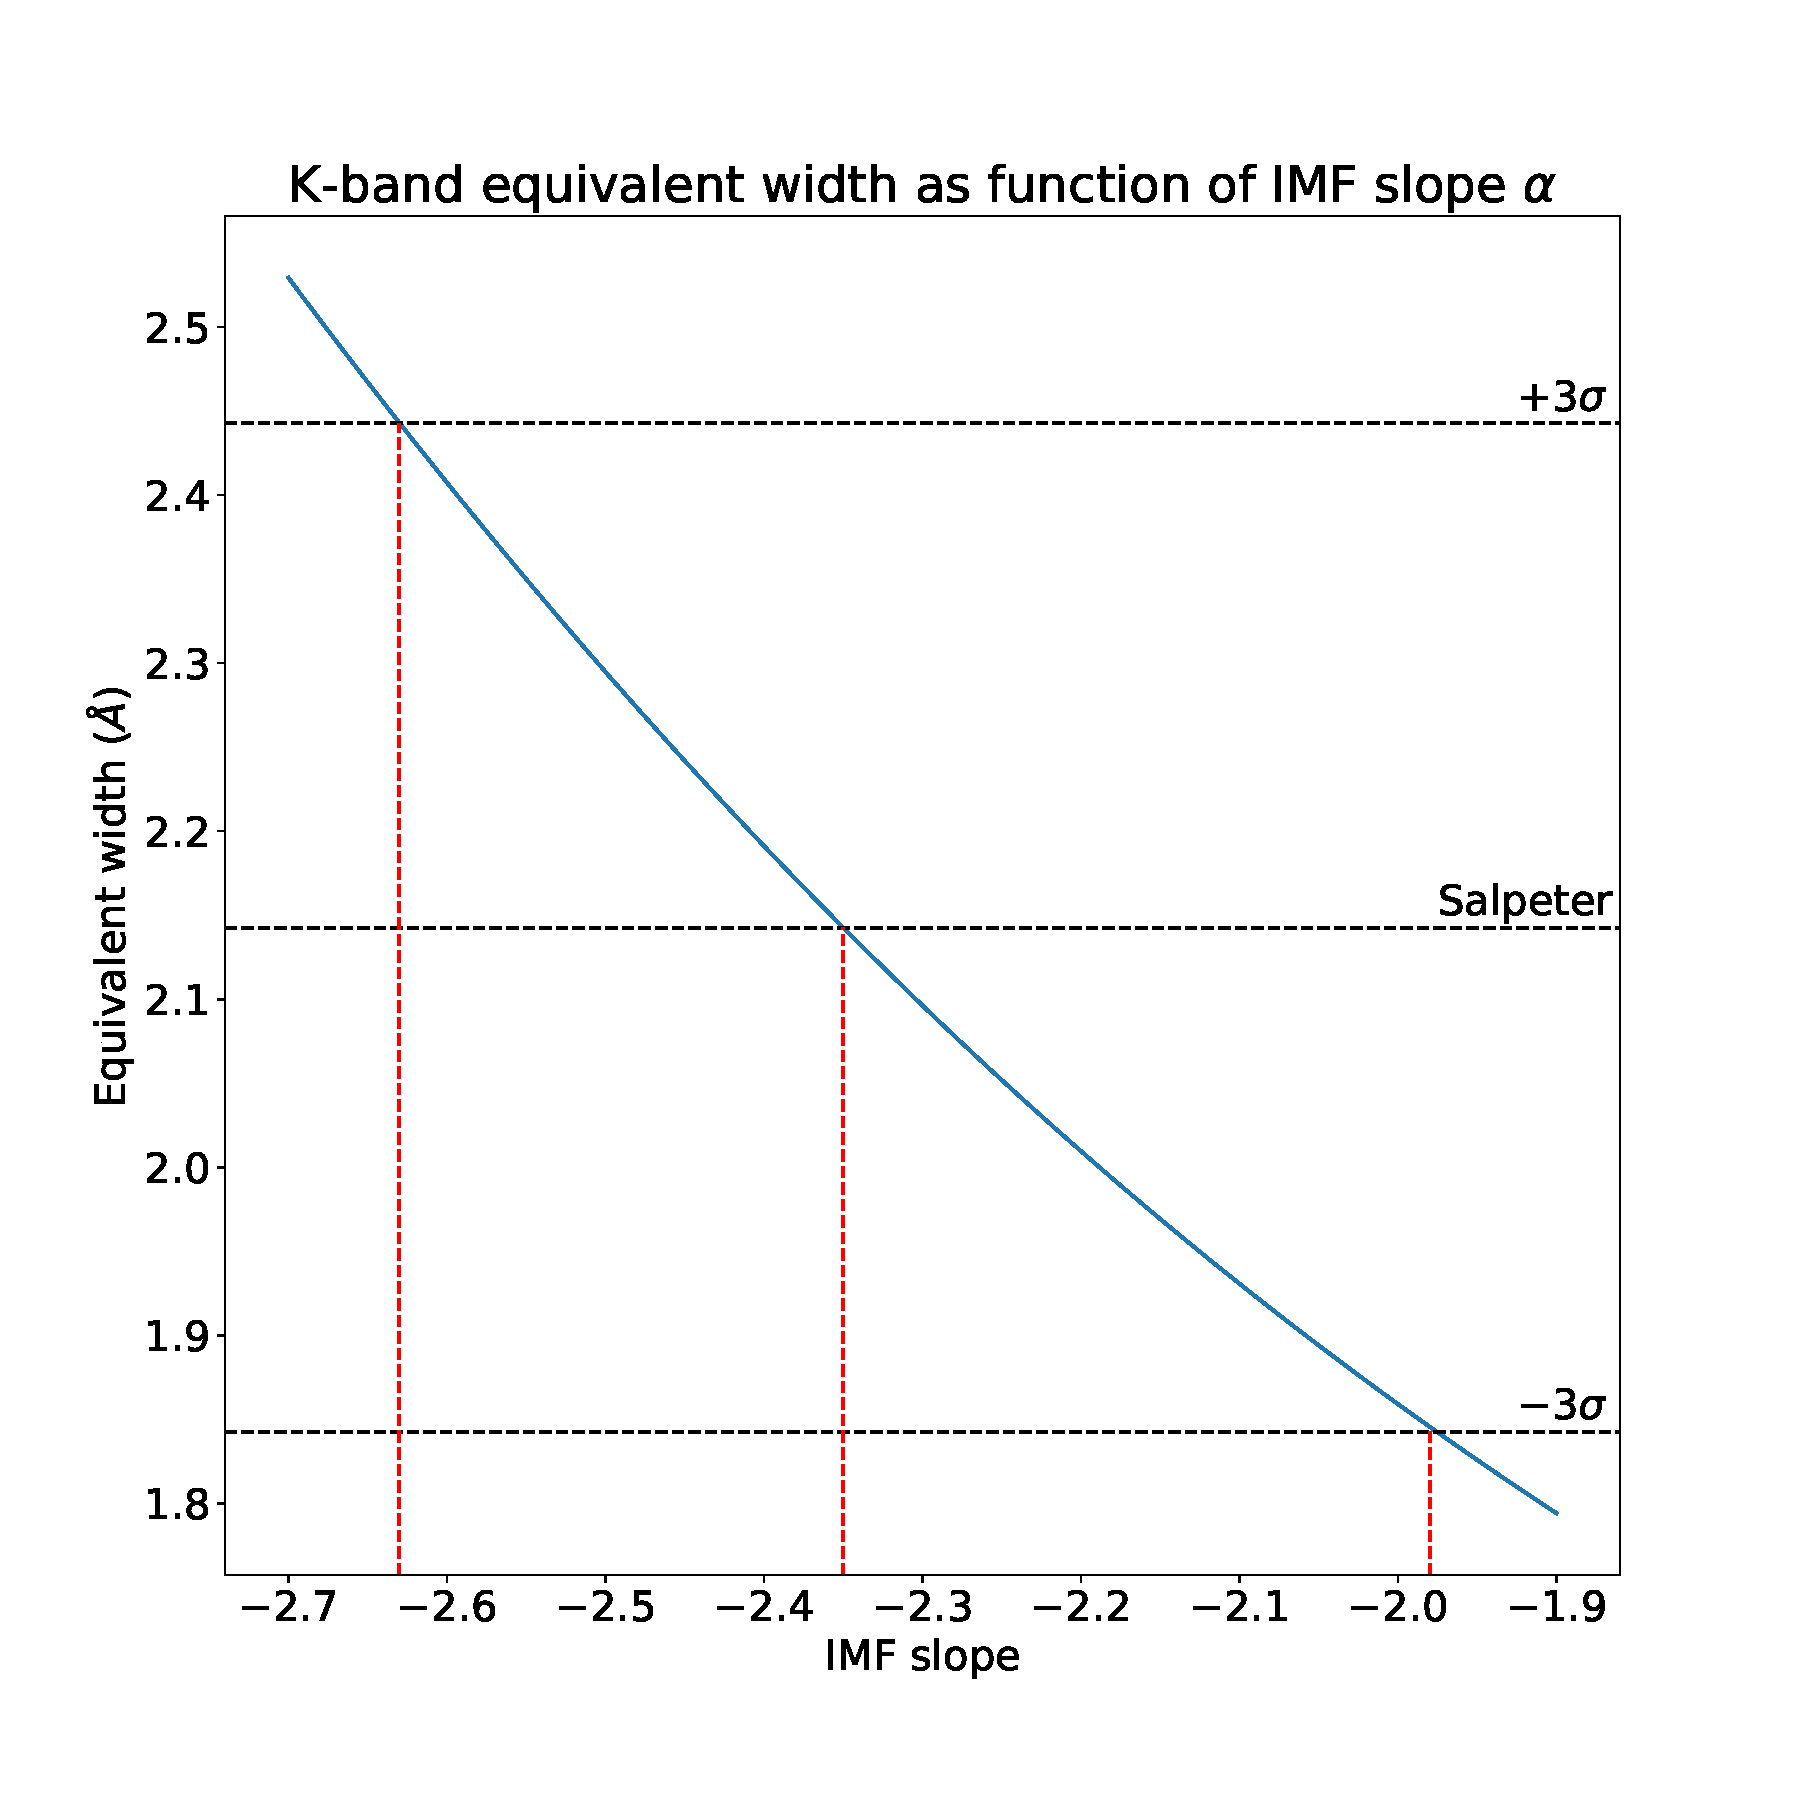
\includegraphics[width=\textwidth]{imf_slope_3sigma.pdf}
  \caption{}
  \label{fig:alpha}
\end{figure}

\end{document}